\chapter*{2021年\textsf{HDU}「大学物理1」期中试题解答}

\begin{minipage}{0.32\textwidth}
    \textbf{开课学院}：理学院
      
    \textbf{课程编码}：A0715011
\end{minipage}
\hfill
\begin{minipage}{0.32\textwidth}
    \textbf{解析制作}：\textsf{M.Xia@WeYoung}

    \textbf{\,\hologo{TeX}~排版}：\textsf{M.Xia}
\end{minipage}
\hfill
\begin{minipage}{0.15\textwidth}
    \centering
    \begin{tikzpicture}
        \node [inner sep=0] at (0,0) {
            \qrcode[height=3em,version=4]{https://qm.qq.com/q/mgD30uPiSs}};
        \fill [color=white,rounded corners=(sqrt(2)+2)/11*1em] (-.5em,-.5em) rectangle (.5em,.5em);
        \node [inner sep=0] at (0,0) {\color{MidnightBlue}\scriptsize\faIcon{qq}};
    \end{tikzpicture}

    \scriptsize\href{https://qm.qq.com/q/mgD30uPiSs}{\itshape 未央物理营}
\end{minipage}
\hfill
\begin{minipage}{0.15\textwidth}
    \centering
    \begin{tikzpicture}
        \node [inner sep=0] at (0,0) {
            \qrcode[height=3em,version=4]{http://weixin.qq.com/r/DBIABcHEqgnWKIVmb0eI}};
            \fill [color=white,rounded corners=(sqrt(2)+2)/11*1em] (-.5em,-.5em) rectangle (.5em,.5em);
        \node [inner sep=0] at (0,0) {\color{DarkGreen}\scriptsize\faIcon{weixin}};
    \end{tikzpicture}

    \scriptsize\href{http://weixin.qq.com/r/DBIABcHEqgnWKIVmb0eI}{\itshape 未央学社}
\end{minipage}

\section{选择题（每题3分，共27分）}

\begin{problem}
    某人以速率$v$向西行驶，今有风以相同速率从北偏东$30^{\circ}$方向吹来，试问人感到风从哪个方向吹来
    \begin{tasks}(4)
        \task 北偏东$30^{\circ}$
        \task 南偏东$30^{\circ}$
        \task[\true] 北偏西$30^{\circ}$
        \task 西偏南$30^{\circ}$
    \end{tasks}
\end{problem}
\solute1
\begin{paracol}{2}
\begin{solution}
    人感到风从哪个方向吹来，即求风相对人的速度$\bm v_{\text{风}\to\text{人}}$.由相对运动关系得
    \[\bm v_{\text{风}\to\text{人}}=\bm v_{\text{风}\to\text{地}}-\bm v_{\text{人}\to\text{地}}\]
    根据上式画出矢量图可知人感到风从北偏西$30^{\circ}$吹来.
    \switchcolumn\vspace*{\fill}\centering
    \begin{tikzpicture}
        \draw [->] (0,0) -- (1,{-sqrt(3)}) node [anchor=north] {$\bm v_{\text{风}\to\text{人}}$};
        \draw [->] (0,0) -- (-1,{-sqrt(3)});
        \draw [->] (1,{-sqrt(3)}) -- (-1,{-sqrt(3)}) node [anchor=north] {$\bm v_{\text{人}\to\text{地}}$} node [anchor=south east] {$\bm v_{\text{风}\to\text{地}}$};
    \end{tikzpicture}\vspace*{\fill}
\end{solution}
\end{paracol}

\begin{problem}
    关于电场强度定义式$\bm E=\bm F/q$，下列说法中哪个是正确的
    \begin{tasks}
        \task 场强$\bm E$的大小与试探电荷$q_0$的大小成反比
        \task[\true] 对场中某点，试探电荷受力$\bm F$与$q_0$的比值不因$q_0$而变
        \task 试探电荷受力$\bm F$的方向就是场强$\bm E$的方向就是场强
        \task 若场中某点不放试探电荷$q_0$，则$\bm F=0$，从而$\bm E=0$
    \end{tasks}
\end{problem}
\begin{solution}
    电场强度只和场源电荷有关，所以A、D错误，B正确；若试探电荷带负电，其受力方向会与场强方向相反，所以C错误.
\end{solution}

\begin{problem}
    一质点在平面上运动，质点位置矢量的表示式为$\bm r=at^2\bm i+bt^2\bm j$（其中$a$，$b$为常量），则该质点作
    \begin{tasks}(4)
        \task 匀速直线运动
        \task[\true] 变速直线运动
        \task 抛物线运动
        \task 一般曲线运动
    \end{tasks}
\end{problem}
\solute0
\begin{solution}
    质点的速率$\abs{\bm v}=\abs{\d\bm r/\d t}=\sqrt{(2at)^2+(2bt)^2}=2\sqrt{a^2+b^2}t$随着时间不断增大；质点的位矢方向$\tan{\theta}=a/b$为一常数，所以质点做变速直线运动.
\end{solution}

\begin{problem}
    一带电体可作为点电荷处理的条件是
    \begin{tasks}(3)
        \task 电荷必须呈球形分布
        \task 带电体的线度很小
        \task 电量很小
        \task![\true] 带电体的线度与其它有关长度相比可忽略不计
    \end{tasks}
\end{problem}

\begin{problem}
    两辆小车$A$、$B$在光滑平直轨道上运动. 第一次实验，$B$静止，$A$以$v_{A_1}=\qty{0.5}{\m/\s}$的速率向右与$B$碰撞，其结果$A$以$v_{A_2}=\qty{0.1}{\m/\s}$的速率弹回，$B$以$v_{B_2}=\qty{0.3}{\m/\s}$的速率向右运动；第二次实验，$B$仍静止，$A$装上$\qty1\kg$的物体后仍以$v_{A_1}'=\qty{0.5}{\m/\s}$的速率与$B$碰撞，结果$A$静止，$B$以$v_{B_2}'=\qty{0.5}{\m/\s}$的速率向右运动. 则$A$和$B$的质量分别为
    \begin{tasks}(2)
        \task $m_A=\qty2\kg$，$m_B=\qty1\kg$
        \task[\true] $m_A=\qty1\kg$，$m_B=\qty2\kg$
        \task $m_A=\qty3\kg$，$m_B=\qty4\kg$
        \task $m_A=\qty4\kg$，$m_B=\qty3\kg$
    \end{tasks}
\end{problem}
\solute2
\begin{solution}
    由碰撞时二者水平方向动量守恒$m_A\times v_{A_1}=-m_A\times v_{A_2}+m_B\times v_{B_2}$，$(m_A+\qty1\kg)\times v_{A_1}'=m_B\times v_{B_2}'$得$m_A=\qty1\kg$，$m_B=\qty2\kg$.
\end{solution}

\begin{problem} % {转动定律}
一轻绳绕在有水平轴的定滑轮上，滑轮的转动惯量为$I$，绳下端挂一物体. 物体所受重力为$P$，滑轮的角加速度为$\beta$. 若将物体去掉而以$P$相等的力直接向下拉绳子，滑轮的角加速度$\beta$将
\begin{tasks}(5)
    \task 不变
    \task 变小
    \task[\true] 变大
    \task* 如何变化无法判断
\end{tasks}
\end{problem}
\solute2
\begin{note}\leavevmode
\begin{itemize}
    \item 下落过程中物体也要增加自己的动能，所以会``拖累''滑轮的加速转动过程. 所以直接用拉力$P$去拉绳子使滑轮获得的角加速度要比重物带着绳子使滑轮获得的角加速度大.
    \item 重物加速下落的过程中属于失重过程，绳子的拉力一定小于其重力$P$，进而拉力对滑轮的力矩就小于$PR$，所以前者角加速度要比后者小，即直接用拉力$P$去拉绳子使滑轮获得的角加速度要比重物带着绳子使滑轮获得的角加速度大.
\end{itemize}
\end{note}
\begin{solution}
设绳子拉力为$T$. 对重物列牛顿运动定律、对滑轮列转动定律得
\[\begin{dcases}
    mg-T=ma\\
    TR=I\beta
\end{dcases}\]
由线量和角量之间的关系$a=R\beta$联立以上两式得$\beta=mgR/(mR^2+I)<mgR/I=PR/I$.
\end{solution}

\begin{paracol}{2}
\begin{problem}
    如图所示，一静止的均匀细棒，长为$L$，质量为$M$，可绕通过棒的端点且垂直于棒长的光滑固定轴$O$在水平面内转动，转动惯量为$ML^2/3$. 一质量为$m$，速率为$v$的子弹在水平面内沿与棒垂直的方向射出并穿出棒的自由端. 设穿过棒后子弹的速率为$v/2$，则此时棒的角速度应为
    \begin{tasks}(4)
        \task $\dfrac{mv}{ML}$
        \task[\true] $\dfrac{3mv}{2ML}$
        \task $\dfrac{5mv}{3ML}$
        \task $\dfrac{7mv}{4ML}$
    \end{tasks}
    \switchcolumn\vspace*{\fill}
    \begin{figure}[htbp]
        \centering
        \begin{tikzpicture}
            \draw (0,.1) rectangle (4,-.1);
            \filldraw (.1,0) circle (.05);
            \node [anchor=north] at (0,-.1) {$O$};
            \draw [very thick,->] (3.9,-1) -- (3.9,-.2) node [near end,right] {$\bm v$};
            \draw [very thick,->] (3.9,.2) -- (3.9,1) node [near end,right] {$\bm v/2$};
        \end{tikzpicture}
        \caption*{俯视图}
    \end{figure}
    \vspace*{\fill}
\end{problem}
\end{paracol}
\solute0
\begin{solution}
    子弹和棒构成的系统对$O$点角动量守恒$mvL=\omega ML^2/3+mvL/2$得$\omega=3mv/2ML$.
\end{solution}

\begin{problem} % 角量与线量的关系
    一刚体以每分钟$60$转绕$z$轴匀速转动（$\omega$沿$z$轴正向）. 某时刻刚体上一点$P$的位置矢量为$r=3\bm i+4\bm j+5\bm k$，单位为``$\qty{e-2}\m$''. 若以``$\qty{e-2}{\m/\s}$''为速度单位，此刻$P$点的速度为
    \begin{tasks}(2)
        \task $\bm v=94.2\bm i+125.6\bm j+157.0\bm k$
        \task[\true] $\bm v=-25.1\bm i+18.8\bm j$
        \task $\bm v=-25.1\bm i-18.8\bm j$
        \task $\bm v=31.4\bm k$
    \end{tasks}
\end{problem}
\solute1
\begin{solution}
    $\bm\omega=60\bm k\unit{r/\min}=2\pi\bm k\unit{\radian/\s}$，$\bm v=\bm\omega\times\bm r=-8\pi\bm i+6\pi\bm j$.
\end{solution}

\begin{problem}
    高斯定理$\oiint_S{\bm E\cdot\d\bm S}=\int_V{\frac{\rho}{\epsilon_0}\d V}$
    \begin{tasks}(2)
        \task[\true] 适用于任何静电场
        \task 只适用于真空中的静电场
        \task! 只适用于具有球对称性、周对称性和平面对称性的静电场
        \task! 只适用于虽然不具有C中所述的对称性、但可以找到合适的高斯面的静电场
    \end{tasks}
\end{problem}

\section{填空题（共23分）}

\begin{problem}
质点沿半径$R$作圆周运动，运动方程为$\theta=2+t^2$ (SI)，则$t$时刻质点法向加速度大小为\ans{$4t^2R$}，角加速度为\ans{$\qty2{\radian/\s^2}$}.
\end{problem}
\solute0
\begin{solution}
    $\omega=\d\theta/\d t=2t$，$a=\omega^2r=4t^2R$，$\beta=\d\omega/\d t=\qty2{\radian/\s^2}$.
\end{solution}

\begin{problem}
    一质点沿$x$轴做直线运动，它的运动学方程为$x=3+5t+6t^2-t^3$ (SI)，则
    \begin{tasks}[label=\arabic*.](2)
        \task 质点在$t=0$时刻的速度$\bm v_0=$\ans{$5\bm i\unit{\m/\s}$}.
        \task 加速度为零时，该质点的速度$v=$\ans{$\qty{17}{\m/\s}$}.
    \end{tasks}
\end{problem}
\solute1
\begin{solution}\leavevmode
\begin{enumerate}
    \item $v=\odv x/t=5+12t-3t^2\xlongequal{t=0}\qty5{\m/\s}$，$a=\d v/\d t=12-6t$.
    \item $a=0$时，$t=\qty2\s$. $v(2)=5+12\times 2-3\times 2^2=\qty{17}{\m/\s}$.
\end{enumerate}
\end{solution}

\begin{paracol}{2}
\begin{problem}
    如图所示，一个小物体$A$靠在一辆小车的竖直前壁上，$A$和车壁间的静摩擦系数是$\mu$. 若要使物体$A$不至掉下来，小车的加速度的最小值应为$a=$\ans{$g/\mu$}.
    \switchcolumn\vspace*{\fill}\centering
    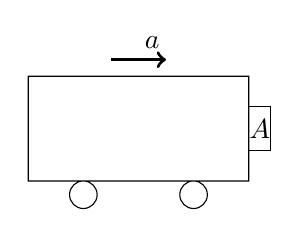
\begin{tikzpicture}[scale=.7]
        \wall{(-3,0)}{(3,-.2)};
        \draw (1,.25) circle (.25) (-1,.25) circle (.25) (-2,.5) rectangle (2,2.4) ;
        \draw [very thick,->] (-.5,2.7) -- (.5,2.7) node [near end,above] {$\bm a$};
        \draw (2,1.05) rectangle (2.4,1.85) node [midway] {$A$};
    \end{tikzpicture}\vspace*{\fill}
\end{problem}\switchcolumn
\solute1
\begin{solution}
    物块与车一同加速，车壁对物块的压力大小为$N=ma$. 物块不掉落，摩擦力需至少等于重力$f=mg$. 代入滑动临界的条件$f=\mu N$得$a=g/\mu$.
\end{solution}
\end{paracol}

\begin{problem}
    地球的质量为$m$，太阳的质量为$M$，地心与日心的距离为$R$，引力常量$G$，则地球绕太阳作圆周运动得轨道角动量$L=$\ans{$m\sqrt{GMR}$}.
\end{problem}
\solute0
\begin{solution}
    引力提供向心力$GMm/R^2=mv^2/R$得$v=\sqrt{GM/R}$. 角动量$L=mvR=m\sqrt{GMR}$.
\end{solution}

\begin{paracol}{2}
\begin{problem}
    三个平行的“无限大”均匀带电平面，其电荷面密度都是$+\sigma$，如图所示. 则$A$，$B$，$C$，$D$四个区域的电场强度分别为\ans{$E_A=-3\sigma/2\epsilon_0$}，\ans{$E_B=-\sigma/2\epsilon_0$}，\ans{$E_C=\sigma/2\epsilon_0$}，\ans{$E_D=3\sigma/2\epsilon_0$}（设向右为正）.
    \switchcolumn\centering
    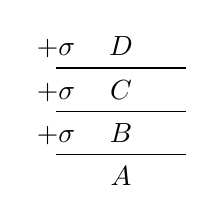
\begin{tikzpicture}[scale=.55,rotate=90]
        \draw (-1,1.5) -- (-1,-1.5);
        \draw (0,1.5) -- (0,-1.5);
        \draw (1,1.5) -- (1,-1.5);
        \node [anchor=south] at (-1,1.5) {$+\sigma$};
        \node [anchor=south] at (0,1.5) {$+\sigma$};
        \node [anchor=south] at (1,1.5) {$+\sigma$};
        \node at (-1.5,0) {$A$};
        \node at (-.5,0) {$B$};
        \node at (.5,0) {$C$};
        \node at (1.5,0) {$D$};
    \end{tikzpicture}
\end{problem}
\end{paracol}
\solute4
\begin{solution}
    由无限大带电平面附近的场强表达式$E_0=\sigma/2\epsilon_0$得
\begin{itemize}
    \item $A$区域的场强由三个右侧的带电平面产生，大小为$-3E_0=-3\sigma/2\epsilon_0$.
    \item $B$区域的场强由一个左侧的和两个右侧的带电平面产生，大小为$E_0-2E_0=-\sigma/2\epsilon_0$.
    \item $C$区域的场强由两个左侧的和一个右侧的带电平面产生，大小为$2E_0-E_0=\sigma/2\epsilon_0$.
    \item $D$区域的场强由三个左侧的带电平面产生，大小为$3E_0=3\sigma/2\epsilon_0$.
\end{itemize}
\end{solution}

\begin{paracol}{2}
    \begin{problem} % {角动量守恒}
        一根长为$l$的细绳的一段固定于光滑水平面上的$O$点，另一端系一质量为$m$的小球，开始时绳子是松弛的，小球与$O$点的距离为$h$. 使小球以某个初速率沿该光滑水平面上一直线运动，该直线垂直于小球初始位置与$O$的连线. 当小球与$O$点的距离达到$l$时，绳子绷紧而使小球沿着另一个以$O$点为圆心的圆形轨道运动，则小球作圆周运动时的动能$E_k$与初动能$E_{k_0}$的比值$E_k/E_{k_0}=$\ans{$h^2/l^2$}.
        \switchcolumn\vspace*{\fill}\centering
        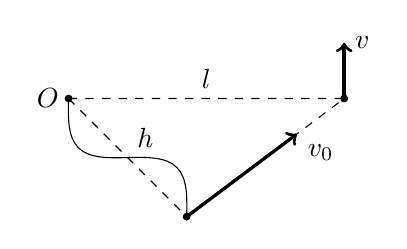
\begin{tikzpicture}
            \draw [dashed] (0,0) -- (1.5,-1.5) node [midway,above right] {$h$} -- (3.5,0) -- cycle node [midway,above] {$l$};
            \draw [very thick,->] (1.5,-1.5) --++ ({1.75*cos(atan(3/4))},{1.75*sin(atan(3/4))}) node [below right] {$v_0$};
            \draw [very thick,->] (3.5,0) --++ (0,{sqrt(2)/2}) node [right] {$v$};
            \draw [rotate around={-45:(0,0)}] (0,0) sin ({.375*sqrt(2)},{-sqrt(2)/4}) cos ({.75*sqrt(2)},0) sin ({1.125*sqrt(2)},{sqrt(2)/4}) cos ({1.5*sqrt(2)},0);
            \fill (0,0) circle (.05) node [left] {$O$};
            \shade [ball color=black] (1.5,-1.5) circle (.05) (3.5,0) circle (.05);
        \end{tikzpicture}\vspace*{\fill}
    \end{problem}
\end{paracol}
\solute2
\begin{solution}
    由于绳子绷紧后拉力始终指向$O$点，故小球对$O$点角动量守恒，即$mv_0h=mvl$. 由于动能和速度平方成正比，所以动能之比为$E_k/E_{k_0}=v^2/v_0^2=h^2/l^2$.
\end{solution}

\begin{problem}
    一半径为$R$，长为$L$的均匀带电圆柱面，其单位长度带有电荷$\lambda$. 在带电圆柱的中垂面上有一点$P$，它到轴线距离为$r$（$r\gg R$），则当$r\ll L$时，$P$点的电场强度的大小$E$=\ans{$\lambda/2\pi\epsilon_0r$}；当$r\gg L$时，$P$点的电场强度的大小$E$=\ans{$\lambda L/4\pi\epsilon_0r^2$}.
\end{problem}
\solute2
\begin{solution}
    当$r\ll L$时，带电体可当作无限长带电绝缘体；当$r\gg L$时，带电体可当作点电荷.
\end{solution}
\solute*{为节约资源，本试题计算题部分不提供演算区域，请自备稿纸，或在下页边缘书写.}

\clearpage
\section{计算题（共50分）}

\begin{paracol}{2}
\begin{problem}
    如图，一质点做半径$R=\qty2\m$的圆周运动，$t=0$时质点位于$A$点，然后顺时针运动，运动方程$S=3\pi t^2+\pi t$.
    \begin{enumerate}
        \item 求质点绕行一周所经历的位移、平均速率.
        \item 求质点在$\qty1\s$末的速度和加速度的大小.
    \end{enumerate}
    \switchcolumn\vspace*{\fill}\centering
    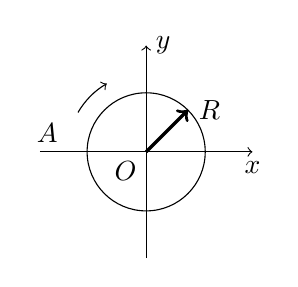
\begin{tikzpicture}[scale=.5]
        \draw (0,0) circle (1.5);
        \draw [->] (-2.7,0) -- (2.7,0) node [below] {$x$};
        \draw [->] (0,-2.7) -- (0,2.7) node [right] {$y$};
        \node [anchor=north east] at (0,0) {$O$};
        \draw [->] ({-2*cos(30)},{2*sin(30)}) arc (150:120:2);
        \node [anchor=south east] at (-2,0) {$A$};
        \draw [very thick,->] (0,0) -- ({1.5/sqrt(2)},{1.5/sqrt(2)}) node [right] {$R$};
    \end{tikzpicture}\vspace*{\fill}
\end{problem}
\end{paracol}
\begin{solution}\leavevmode
    \begin{enumerate}
        \item 质点绕行一周后回到起点，位移为零. 质点绕行一周，经历路程$\Delta S=2\pi R=4\pi\unit\m$. 令$S=\Delta S$得用时$\Delta t=\qty1\s$. 所以平均速率$\overline{v}=\Delta S/\Delta t=4\pi\unit{\m/\s}$.
        \item
        \begin{tasks}[label=\labelitemi](2)
            \task! 质点的速度大小$v=\d s/\d t=6\pi t+\pi\big|_{t=\qty1\s}=7\pi\unit{\m/\s}$.
            \task 切向加速度$a_\tau=\d v/\d t=6\pi\unit{\m/\s}$.
            \task 法向加速度$a_n=v^2/R=49\pi^2/2\unit{\m/\s^2}$.
            \task! 所以质点的加速度为$a=\sqrt{a_{\tau}^2+a_n^2}=\qty{242.54}{\m\cdot\s^{-2}}$.
        \end{tasks}
    \end{enumerate}
\end{solution}

\begin{problem}
    质量为$\qty5\kg$的质点，所受外力$\bm F=2t\bm j$，该质点从$t=0$时刻由静止开始运动. 求前$\qty3\s$内，外力所做的功.
\end{problem}
\begin{solution}\leavevmode
    \begin{itemize}
        \item 质点的加速度为$a=F/m=0.4t$. 积分得质点的速度$v=\int_0^t{0.4 t\d t}=0.2t^2$.
        \item 所以前$\qty3\s$内外力所做的功为$W=\int_0^3F\d x=\int_0^3Fv\d t\int_0^3{2t\cdot 0.2t^2\d t}=\qty{8.1}\J$.
    \end{itemize}
\end{solution}

\begin{problem}
    设想有两个自由质点，其质量分别为$m_1$和$m_2$，它们之间的相互作用符合万有引力定律. 开始时，两质点间的距离为$l$，它们都处于静止状态. 试求当它们的距离变为$l/2$时，两质点的速度各为多少.
\end{problem}
\begin{solution}
    设两质点的速度大小分别为$v_1$和$v_2$. 由动量守恒、机械能守恒分别有
    \[\begin{dcases}
        m_1v_1+m_2v_2=0\\
        -\frac{Gm_1m_2}{l}=\frac12m_1v_1^2+\frac12m_2v_2^2-\frac{Gm_1m_2}{l/2}
    \end{dcases}\]
    联立两式得
    \[v_1=m_2\sqrt{\frac{2G}{(m_1+m_2)l}},\ v_2=-m_1\sqrt{\frac{2G}{(m_1+m_2)l}}\]
    负号代表两质点的速度方向相反.
\end{solution}

\begin{problem}
    设两个粒子之间的相互作用力是排斥力，其大小与粒子间距离$r$的函数关系为$f=k/r^3$，$k$为正值常量. 试求两个粒子相距为$r$时的势能（设相互作用力为零的地方势能为零）.
\end{problem}
\begin{solution}
    无穷远处相互作用力为零，势能为零. $E=\int_r^{\infty}{f\d r}=k/2r^2$.
\end{solution}

\begin{problem}
\begin{paracol}{2}
    在强度的大小为$E$，方向竖直向上的匀强电场中，有一半径为$R$的半球形光滑绝缘槽放在光滑水平面上（如图所示）. 槽的质量为$M$，一质量为$m$带有电荷$+q$的小球从槽的顶点$A$处由静止释放. 如果忽略空气阻力且质点受到的重力大于其所受电场力，求
\switchcolumn\centering
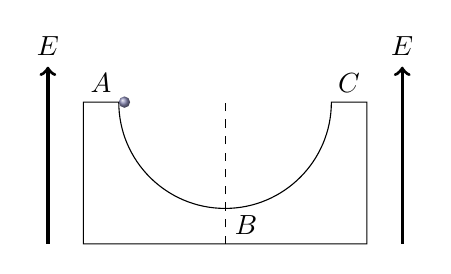
\begin{tikzpicture}[scale=.9]
    \wall{(-3,0)}{(3,-.3)};
    \draw (-2,2) -- (-1.5,2) node [midway,above] {$A$} arc (-180:0:1.5) -- (2,2) node [midway,above] {$C$} -- (2,0) -- (-2,0) node [midway,above right] {$B$} -- cycle;
    \draw [very thick,->] (-2.5,0) -- (-2.5,2.5) node [above] {$\bm E$};
    \draw [very thick,->] (2.5,0) -- (2.5,2.5) node [above] {$\bm E$};
    \draw [dashed] (0,0) -- (0,2);
    \shade [ball color=MidnightBlue!50] (-1.42,2) circle (.08);
\end{tikzpicture}
\end{paracol}
\begin{enumerate}
    \item 小球由顶点$A$滑至半球最低点$B$时相对地面的速度.
    \item 小球通过$B$点时，槽相对地面的速度，小球能否再上升到右端最高点$C$.
\end{enumerate}
\end{problem}
\begin{solution}
    设在$B$点小球与槽的速度大小分别为$v_1$和$v_2$. 由动量守恒、机械能守恒分别有
    \[\begin{dcases}
        mv_1+Mv_2=0\\
        mgR-qER=\frac12mv_1^2+\frac12Mv_2^2
    \end{dcases}\]
    联立以上两式得
    \[v_1=\sqrt{\frac{2MR(mg-qE)}{m^2+Mm}},\ v_2=-\sqrt{\frac{2mR(mg-qE)}{M^2+Mm}}\]
    负号表示速度方向水平向左. 由于没有非保守力做功，所以小球可以再升到$C$点.
\end{solution}

\begin{problem}
    质量为$\qty{75}\kg$的人站在半径为$\qty2\m$的水平转台边缘. 转台的固定转轴竖直通过台心且无摩擦. 转台绕竖直轴的转动惯量为$\qty{3000}{\kg\cdot\m^{-2}}$. 开始时整个系统静止. 现人以相对于地面为$\qty1{\m/\s}$的速率沿转台边缘行走. 求人沿转台边缘行走一周，回到他在转台上初始位置所用的时间.
\end{problem}
\begin{solution}
    人相对地面的角速度$\omega=v/R$. 转轴没有摩擦，由人和转台角动量守恒$mR^2\omega+I\omega'=0$得转台的角速度$\omega'=-mvR/I=\qty{-0.05}{\radian/\s}$. 人相对转台的角速度为$\omega_r=\omega-\omega'=\qty{0.55}{\radian/\s}$，走动一圈的角位移$\Delta\theta=2\pi$，所用时间为$t=2\pi/\omega_r=2\pi/{0.55}=\qty{11.4}\s$.
\end{solution}

\begin{paracol}{2}
\begin{problem}
    两个电量分别为$q_1=\qty{2e-7}\C$和$q_2=\qty{-2e-7}\C$的点电荷，相距$\qty{0.3}\m$. 求距$q_1$为$\qty{0.4}\m$，距$q_2$为$\qty{0.5}\m$处$P$点电场强度.
\end{problem}
\begin{solution}
    $P$点场强由$q_1$和$q_2$在$P$点的场强的矢量叠加，二者分别为
    \[\bm E_1=\frac{q_1}{4\pi\epsilon_0b^2}(-\bm j),\ \bm E_2=\frac{\abs{q_2}}{4\pi\epsilon_0c^2}\cos\alpha\bm i+\frac{\abs{q_2}}{4\pi\epsilon_0c^2}\sin\alpha\bm j\]
    故$P$点场强为$\bm E=\bm E_1+\bm E_2=4320\bm i-5490\bm j$.
\end{solution}
\switchcolumn\vspace*{\fill}\centering
\begin{tikzpicture}[scale=.8]
    \draw [<->] (0,4) node [left] {$y$} -- (0,0) coordinate (o) -- (3,0) node (b) [right] {$x$};
    \draw [dashed] (0,0) -- (2.4,3.2) -- (0,3.2);
    \shade[ball color=MidnightBlue!50] (0,3.2) circle (.1) node [left] {$q_1$};
    \shade[ball color=DarkGreen!50] (2.4,3.2) circle (.1) node (a) [right] {$q_2$};
    \draw [very thick,<->] (.48,.64) node [above] {$E_2$} -- (0,0) node [left] {$P$} -- (0,-1) node [left] {$E_1$};
    \pic["$\alpha$", draw=DarkRed, very thick, angle eccentricity=1.5, angle radius=12]{angle=b--o--a};
\end{tikzpicture}\vspace*{\fill}
\end{paracol}